\documentclass[tikz, border=5pt]{standalone}
\usepackage{tikz}
\usetikzlibrary{shapes.geometric, arrows}

\tikzstyle{startstop} = [rectangle, rounded corners, minimum width=3cm, minimum height=1cm,text centered, draw=black, fill=red!30]
\tikzstyle{process} = [rectangle, minimum width=3cm, minimum height=1cm, text centered, draw=black, fill=blue!20]
\tikzstyle{decision} = [diamond, minimum width=3cm, minimum height=1cm, text centered, draw=black, fill=yellow!30]
\tikzstyle{arrow} = [thick,->,>=stealth]

\tikzstyle{block} = [rectangle, minimum width=3.5cm, minimum height=1.2cm, text centered, draw=black, fill=blue!20]
%\tikzstyle{data} = [parallelogram, minimum width=3.5cm, minimum height=1.2cm, text centered, draw=black, fill=green!20]
\tikzstyle{data} = [trapezium, trapezium angle=75, minimum width=3.5cm, minimum height=1.2cm, text centered, draw=black, fill=green!20]
\tikzstyle{command} = [rectangle, minimum width=3cm, minimum height=0.8cm, text centered, draw=black, fill=green!20]

\begin{document}
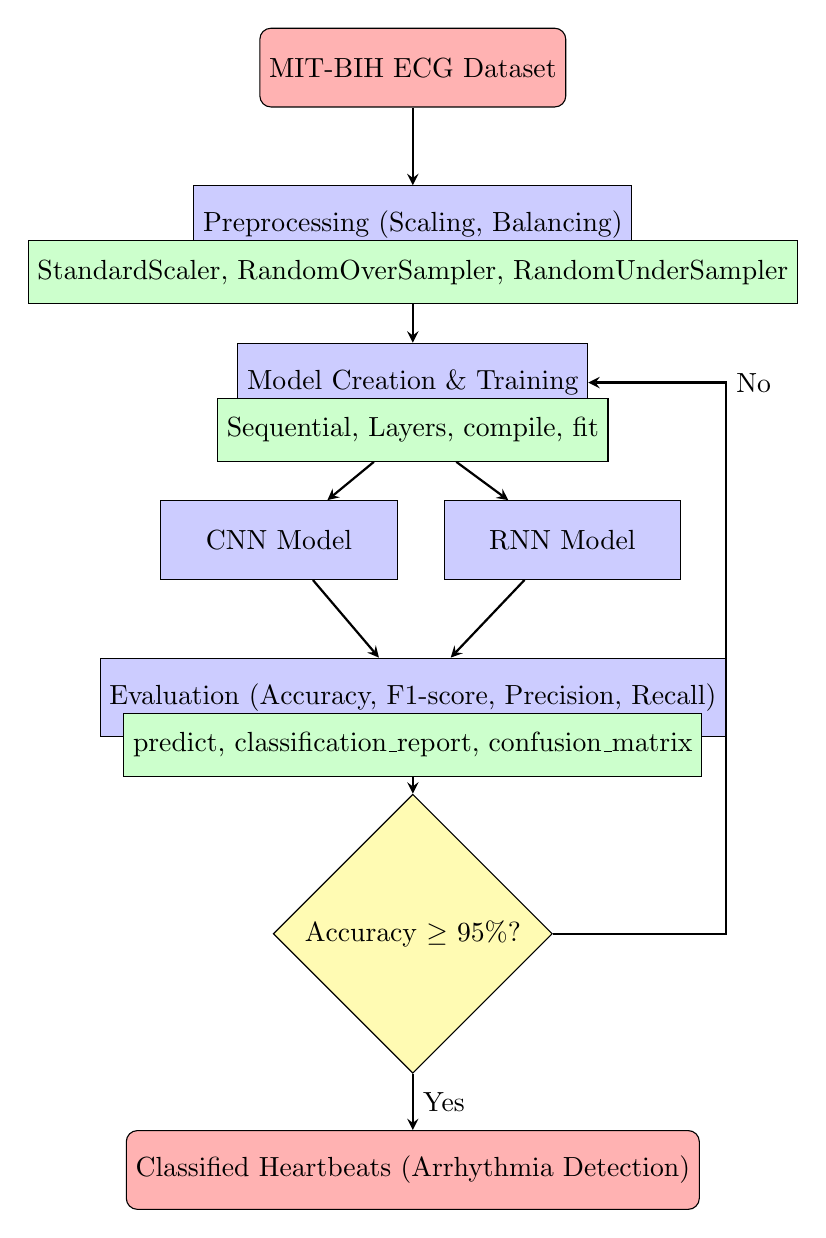
\begin{tikzpicture}[node distance=2cm]
    % Nodes
    \node (input) [startstop] {MIT-BIH ECG Dataset};
    \node (preprocess) [process, below of=input] {Preprocessing (Scaling, Balancing)};
    \node (training) [process, below of=preprocess] {Model Creation \& Training};
    \node (cnn) [process, below of=training, xshift=-1.7cm] {CNN Model};
    \node (rnn) [process, right of=cnn, xshift=1.6cm] {RNN Model};
    %\node (fusion) [process, below of=cnn] {Model Fusion (Ensemble or Best Model)};
    \node (evaluation) [process, below of=cnn, xshift=1.7cm] {Evaluation (Accuracy, F1-score, Precision, Recall)};
    \node (decision) [decision, below of=evaluation, yshift=-1cm] {Accuracy $\geq$ 95\%?};
    \node (output) [startstop, below of=decision, yshift=-1cm] {Classified Heartbeats (Arrhythmia Detection)};

    % Commands and data flow
    \node (cmd-preprocess) [command, right of=preprocess, yshift=-0.6cm, xshift=-2cm] {StandardScaler, RandomOverSampler, RandomUnderSampler};
    \node (cmd-training) [command, right of=training, yshift=-0.6cm, xshift=-2cm] {Sequential, Layers, compile, fit};
    \node (cmd-evaluation) [command, right of=evaluation, yshift=-0.6cm, xshift=-2cm] {predict, classification\_report, confusion\_matrix};
    
    % Arrows
    \draw [arrow] (input) -- (preprocess);
    \draw [arrow] (cmd-preprocess) -- (training);
    \draw [arrow] (cmd-training) -- (cnn);
    \draw [arrow] (cmd-training) -- (rnn);
    \draw [arrow] (cnn) -- (evaluation);
    \draw [arrow] (rnn) -- (evaluation);
    \draw [arrow] (cmd-evaluation) -- (decision);
    \draw [arrow] (decision.east) -- ++(2.2,0) |- (training.east) node[midway, right] {No};
    \draw [arrow] (decision) -- (output) node[midway, right] {Yes};
\end{tikzpicture}

\end{document}